% diag_training: TikZ twin of paper/figures/diag_training.pdf (generated by diag_common.py).
% Coordinates are inches (y up). Needs \usepackage{tikz}. Body font 7 pt.
\definecolor{dgA}{HTML}{F0F0F0}\definecolor{dgB}{HTML}{DCDCDC}\definecolor{dgC}{HTML}{C4C4C4}
\definecolor{dgAtk}{HTML}{F2C9B8}\definecolor{dgHw}{HTML}{E3EEF7}
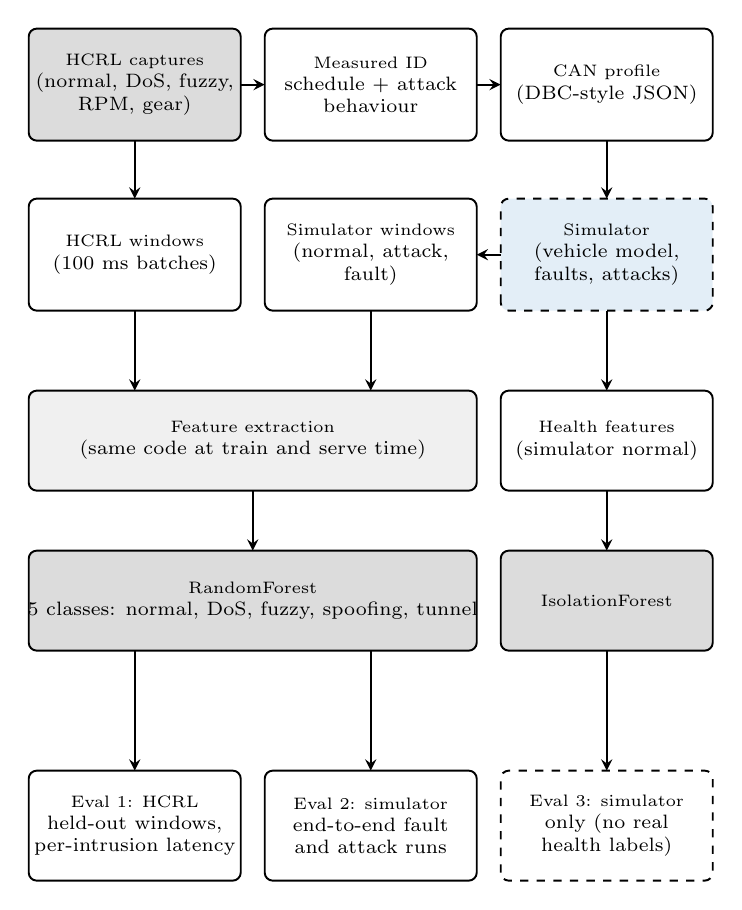
\begin{tikzpicture}[x=1in,y=1in,>=stealth,font=\fontsize{7}{8}\selectfont,line width=0.7pt]
\draw[rounded corners=2.9pt,fill=dgB,line width=0.7pt] (0.040,3.750) rectangle (1.100,4.310);
\node[align=center,inner sep=0pt] at (0.570,4.030) {\fontsize{6.5}{7.3}\selectfont HCRL captures\\ (normal, DoS, fuzzy,\\ RPM, gear)};
\draw[rounded corners=2.9pt,fill=white,line width=0.7pt] (1.220,3.750) rectangle (2.280,4.310);
\node[align=center,inner sep=0pt] at (1.750,4.030) {\fontsize{6.5}{7.3}\selectfont Measured ID\\ schedule + attack\\ behaviour};
\draw[rounded corners=2.9pt,fill=white,line width=0.7pt] (2.400,3.750) rectangle (3.460,4.310);
\node[align=center,inner sep=0pt] at (2.930,4.030) {\fontsize{6.5}{7.3}\selectfont CAN profile\\ (DBC-style JSON)};
\draw[->,line width=0.8pt] (1.100,4.030) -- (1.220,4.030);
\draw[->,line width=0.8pt] (2.280,4.030) -- (2.400,4.030);
\draw[rounded corners=2.9pt,fill=dgHw,line width=0.7pt,dashed] (2.400,2.900) rectangle (3.460,3.460);
\node[align=center,inner sep=0pt] at (2.930,3.180) {\fontsize{6.5}{7.3}\selectfont Simulator\\ (vehicle model,\\ faults, attacks)};
\draw[->,line width=0.8pt] (2.930,3.750) -- (2.930,3.460);
\draw[rounded corners=2.9pt,fill=white,line width=0.7pt] (0.040,2.900) rectangle (1.100,3.460);
\node[align=center,inner sep=0pt] at (0.570,3.180) {\fontsize{6.5}{7.3}\selectfont HCRL windows\\ (100 ms batches)};
\draw[->,line width=0.8pt] (0.570,3.750) -- (0.570,3.460);
\draw[rounded corners=2.9pt,fill=white,line width=0.7pt] (1.220,2.900) rectangle (2.280,3.460);
\node[align=center,inner sep=0pt] at (1.750,3.180) {\fontsize{6.5}{7.3}\selectfont Simulator windows\\ (normal, attack,\\ fault)};
\draw[->,line width=0.8pt] (2.400,3.180) -- (2.280,3.180);
\draw[rounded corners=2.9pt,fill=dgA,line width=0.7pt] (0.040,2.000) rectangle (2.280,2.500);
\node[align=center,inner sep=0pt] at (1.160,2.250) {\fontsize{6.5}{7.3}\selectfont Feature extraction\\ (same code at train and serve time)};
\draw[->,line width=0.8pt] (0.570,2.900) -- (0.570,2.500);
\draw[->,line width=0.8pt] (1.750,2.900) -- (1.750,2.500);
\draw[rounded corners=2.9pt,fill=dgB,line width=0.7pt] (0.040,1.200) rectangle (2.280,1.700);
\node[align=center,inner sep=0pt] at (1.160,1.450) {\fontsize{6.5}{7.3}\selectfont RandomForest\\ 5 classes: normal, DoS, fuzzy, spoofing, tunnel};
\draw[->,line width=0.8pt] (1.160,2.000) -- (1.160,1.700);
\draw[rounded corners=2.9pt,fill=white,line width=0.7pt] (2.400,2.000) rectangle (3.460,2.500);
\node[align=center,inner sep=0pt] at (2.930,2.250) {\fontsize{6.5}{7.3}\selectfont Health features\\ (simulator normal)};
\draw[->,line width=0.8pt] (2.930,2.900) -- (2.930,2.500);
\draw[rounded corners=2.9pt,fill=dgB,line width=0.7pt] (2.400,1.200) rectangle (3.460,1.700);
\node[align=center,inner sep=0pt] at (2.930,1.450) {\fontsize{6.5}{7.3}\selectfont IsolationForest};
\draw[->,line width=0.8pt] (2.930,2.000) -- (2.930,1.700);
\draw[rounded corners=2.9pt,fill=white,line width=0.7pt] (0.040,0.050) rectangle (1.100,0.600);
\node[align=center,inner sep=0pt] at (0.570,0.325) {\fontsize{6.5}{7.3}\selectfont Eval 1: HCRL\\ held-out windows,\\ per-intrusion latency};
\draw[rounded corners=2.9pt,fill=white,line width=0.7pt] (1.220,0.050) rectangle (2.280,0.600);
\node[align=center,inner sep=0pt] at (1.750,0.325) {\fontsize{6.5}{7.3}\selectfont Eval 2: simulator\\ end-to-end fault\\ and attack runs};
\draw[rounded corners=2.9pt,fill=white,line width=0.7pt,dashed] (2.400,0.050) rectangle (3.460,0.600);
\node[align=center,inner sep=0pt] at (2.930,0.325) {\fontsize{6.5}{7.3}\selectfont Eval 3: simulator\\ only (no real\\ health labels)};
\draw[->,line width=0.8pt] (0.570,1.200) -- (0.570,0.600);
\draw[->,line width=0.8pt] (1.750,1.200) -- (1.750,0.600);
\draw[->,line width=0.8pt] (2.930,1.200) -- (2.930,0.600);
\end{tikzpicture}
